\label{chapter6}
\chapter{Presenting proposed profiles}

Previously defined profiles will be presented in-depth. 
In general, each profile has its use-case already assigned in table x.
Here, we will focus on exposing the main features, issues, and use cases. 

Few things must be defined. Data for profiles below was used from REFIT dataset and building 2.
Data was collected from 2013-09-18 to 2015-05-28.
\section{Time ranges}
One important thing to mention is use cases for different time ranges of load profiles.
Based on table \ref{tab:contributions} it is possible to see that most publications and \ref{tab:use_cases} use daily time range.

Generally daily profiles are easier to build since they do not need as much data as others do.
In order to build a decent profile one needs enough data. Sufficient of data is the amount that covers major events.
For daily profile few weeks of data is enough, weekly load profiles need few months of data, monthly few years and yearly around a decade.
And this is the issue, there is rarely enough data to build such profiles. And even then, usage pattern could change in a long time period such as decade.

Combining that with smaller number of use cases for such profiles, shows why such profiles were not looked into as much.

One more thing about time ranges that needs to be included are patterns that they capture or present.
Daily profiles present daily usage and enable us to extract contextual events such as waking up, cooking, leisure time and so on.
Weekly pattern is also repetitive, and it also enables us to see how appliance usage changes over the week and weekends.
Monthly profile has none of the above. It is not repetitive since each day of month can be different day of week.
Alternatively it could be presented as week in a month, but there is no significant usage pattern to be revealed.
The last is yearly profiled, this one presents the seasonal effects on usage such as increased daylight and temperature. 


\section{Per-house}
In this section we will focus on per-house profiles, meaning whole building usage is presented as a single load profile.
This kind of presentation is useful for observing general activation trends in a building.
Possible use cases for per-house load profiles are in grid management and energy saving.

When it comes to activation load profiles there is one issue compared to power load profiles.
In order to build per-house power load profiles it is possible to use main power meter, whereas in activation load profiles sub-meter data is needed.
This can be solved using NILM algorithms, but they are not in phase of practical use yet.

Daily profile per-house profile is also known as standard load profile. 
According to table \ref{tab:contributions} this is most commonly used power profile.
Figures \ref{fig:SLPdaily2} and \ref{fig:SLPyearly2} present usage patterns on different time ranges. 

\begin{figure}[H]
	\centering
	\caption{"Daily per-house load profile"}
	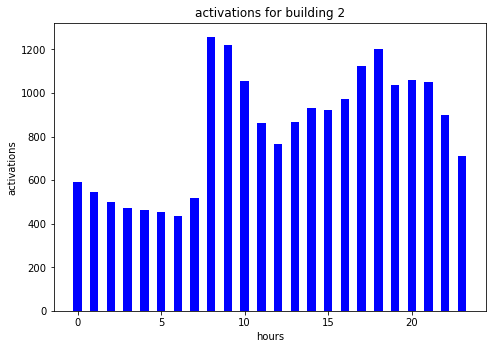
\includegraphics[width=0.9\textwidth]{../Figures/LPS/SLPdaily2.png}
	\label{fig:SLPdaily2}
\end{figure}

\begin{figure}[H]
	\centering
	\caption{"Daily per-house load profile"}
	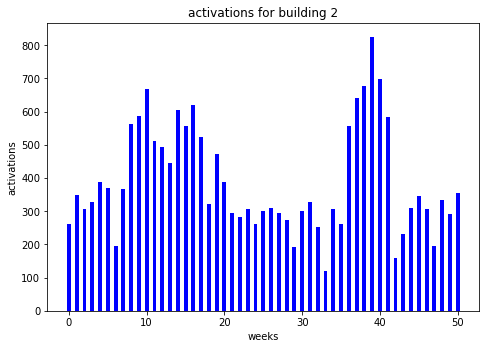
\includegraphics[width=0.9\textwidth]{../Figures/LPS/SLPyearly2.png}
	\label{fig:SLPyearly2}
\end{figure}

\subsection{Per-house two-dimensional time}

Presents more detailed LP compared to daily per house load profile. Use cases are grid management and energy saving.
Example would be load shedding.
Using this LP, ED would disconnect the houses with least activity and highest power consumption. 

Alternatively, it is possible to combine figures \ref{fig:SLPdaily2} and \ref{fig:SLPyearly2} and present
activations as a heat map.
Result is load profile showing more complex usage patterns.

\begin{figure}[H]
	\centering
	\caption{"Yearly per-appliance load profile"}
	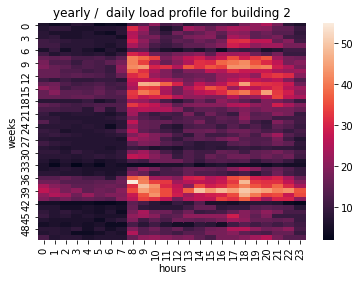
\includegraphics[width=0.9\textwidth]{../Figures/LPS/SLPHMyearly2.png}
	\label{fig:SLPHMyearly2}
\end{figure}

Previously it was mentioned that this kind of profiles are most applicable grid managment and eneregy saving fields. 
One such example could be load shedding.
Using Load profile above, electrical energy providers could find buildings with the least activity at that time of day.
Combining that with power data, it could disconnect the buildings with least activity and most power consumption.


\section{Per-appliance}

Per appliance load profiles offer look into consumption of each individual appliance. 
In this case activation load profiles, this is elemental load profile, since all other 
profiles are built on top of it. 
This also means that it is one of the most universal profiles, since it can be used in all previously defined use cases.
Comparing power and activation profiles in per-house chapter,
it was possible to see that activation does not bring significant advantages over power profiles.
In case of per appliances, it is possible to analyze the usage more in depth.

\begin{figure}[H]
	\centering
	\caption{"Daily per-house load profile"}
	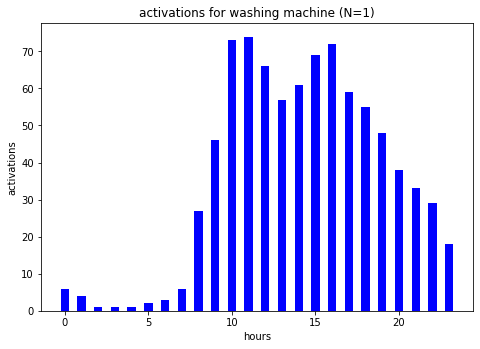
\includegraphics[width=0.9\textwidth]{../Figures/LPS/WM_daily.png}
	\label{fig:WM_daily}
\end{figure}

Another parameter that was not mentioned is the resolution of load profiles. 
Histograms can be presented using various resolutions or number of buckets.
Optimal number of buckets is a number that clearly presents the usage pattern. 

4 hour bucket size on figure \ref{fig:4hours} does a good job at presenting the appliance usage at main parts of the day.
This offers better contextual presentation that is easier to process.

\begin{figure}[H]
	\centering
	\caption{"Daily per-house load profile"}
	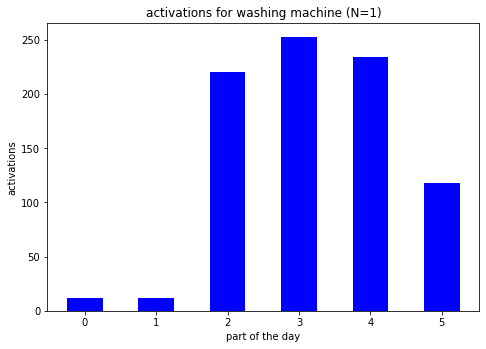
\includegraphics[width=0.9\textwidth]{../Figures/LPS/4 hours.png}
	\label{fig:4hours}
\end{figure}

While low resoltion is usefull for contextual presentation,
high resolution is needed for time-sensitive appliactions as eldery-care,
where we have to detect an accitent as soon as possible.
Hourly resolution would mean that in case of an accident system would need at least an hour to detect it.
While this is sufficient for demonstrating the capabilites, real implementation would need to use lower resolution data.

In case, dwellers have different usage pattern during the weekends, two profiles have to be developed. It is possible 
to present them both at once such as on figure \ref{fig:WM_ww_daily}. This is esentialy a variation of weekly Load
profile that mantains high resolution.

\begin{figure}[H]
	\centering
	\caption{"Daily per-appliance with weekly and weekday load profiles"}
	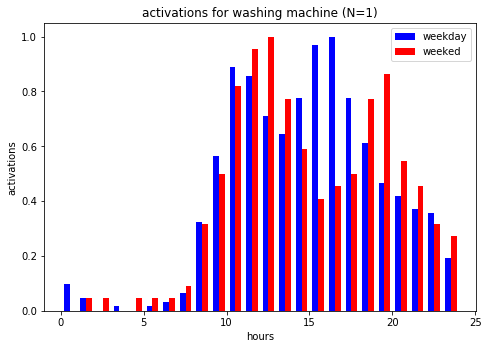
\includegraphics[width=0.9\textwidth]{../Figures/LPS/WM_ww_daily.png}
	\label{fig:WM_ww_daily}
\end{figure}

Another way to present weekly data is figure \ref{fig:WM_weekly}
This resolution offers look into how consumption pattern changes over
the week. This is useful for applications such as grid management and energy saving.
In this particular case it is possible to see that user most commonly uses the washing machine at middle of the week.
Using weekly weather report that would indicate high energy production on wednesday it could offer low cost for energy for that day. 
This kind of presentation could also be used to detect daily anomalies.

\begin{figure}[H]
	\centering
	\caption{"Weekly per-appliance load profile"}
	\includegraphics[width=0.9\textwidth]{../Figures/LPS/WM_weekly.png}
	\label{fig:WM_weekly}
\end{figure}

As mentioned earlier, monthly presentation does not show any significant usage pattern,
yearly presentation again shows the more broad usage pattern.
This is useful for grid management and energy saving,
where one could detect increased usage per appliance, or other trends. 

\begin{figure}[H]
	\centering
	\caption{"Yearly per-appliance load profile"}
	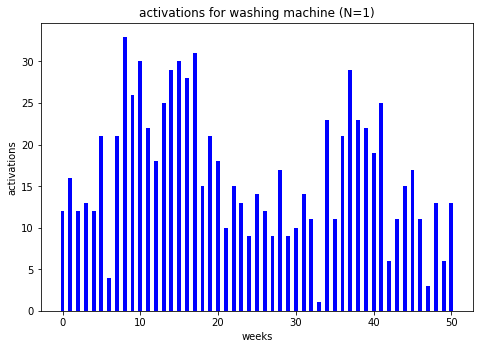
\includegraphics[width=0.9\textwidth]{../Figures/LPS/WM_yearly.png}
	\label{fig:WM_yearly}
\end{figure}


\subsection{Two dimensional time per-appliance load profiles}

Again using a combination of figures \ref{fig:WM_daily} and \ref{fig:WM_weekly},
it is possible to generate a heatmap \ref{fig:wm_hm_weekly}.

\begin{figure}[H]
	\centering
	\caption{"Yearly per-appliance load profile"}
	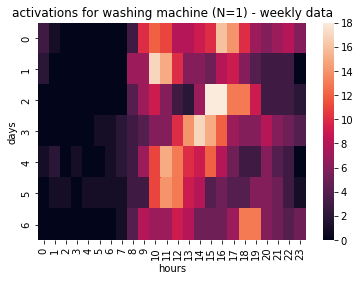
\includegraphics[width=0.9\textwidth]{../Figures/LPS/wm_hm_weekly.png}
	\label{fig:wm_hm_weekly}
\end{figure}

In this case similar use case could be fitted as in first example.
First example used load shedding for when grid is too loaded.
Issues can also occur when grid does not have enough load.
There are two solutions either to decrease the production, which can be slow and expensive.
Other option is to turn on appliances using a control system, or notify users to turn on appliances that they have 
used in the past. 
Due to increasing number of renewable energy sources,
more and more of energy peaks will be weather dependent such as wind and cloud coverage.
By cobining weekly wind forecast, weekly cloud coverage and users consumption profiles energy providers could notify users to turn on the appliances at peak usage time.

By analyzeing figure \ref{fig:wm_hm_weekly} it is possible to see that user uses washing machine,
on wednesdays at 15-16 o clock quite commonly. 
If weather report shoud indicate high production peaks, electrical provider should offer low cost eneregy for that time of day for all users with
similar usage pattern. 
This could all be automated for appliances such  as homegrid batteries, water heaters, EVs or even fridges with a control system.
This would mean that grid operator or electrical distribution company could regulate the demand instantly.
By using load profiles it could prioritise appliances that would be used anyway, which would alse leave minimal impact on users routine. 

\subsubsection{Other two-dimensional presentations}

Figures below show how some appliances have constant usage pattern 
over a year, where again others change it. Examples bellow are randmly picked appliances
from UK-DALE and REFIT. 

\begin{figure}[H]
	\centering
	\caption{"Yearly two-dimensional computer load profile"}
	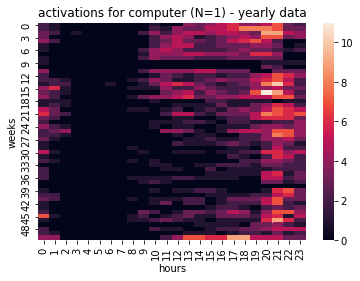
\includegraphics[width=0.9\textwidth]{../Figures/LPS/HM_Ywh_comp.png}
	\label{fig:HM_Ywh_comp}
\end{figure}
\begin{figure}[H]
	\centering
	\caption{"Yearly per-appliance load profile"}
	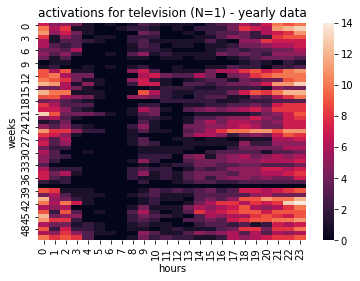
\includegraphics[width=0.9\textwidth]{../Figures/LPS/HM_Ywh_tv.png}
	\label{fig:HM_Ywh_tv}
\end{figure}
\begin{figure}[H]
	\centering
	\caption{"Yearly per-appliance load profile"}
	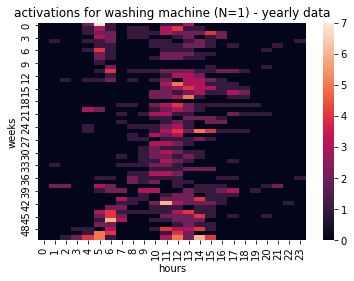
\includegraphics[width=0.9\textwidth]{../Figures/LPS/HM_Ywh_wm.png}
	\label{fig:HM_Ywh_wm}
\end{figure}

another example worth mentioning is one from UK-dale building 1, where data as collected from 2012-11-09 to 2017-04-26.
Roughly 5 years of data means that it is possible to build a decent profile. 

\begin{figure}[H]
	\centering
	\caption{"Yearly two-dimensional solar termal pumping station load profile"}
	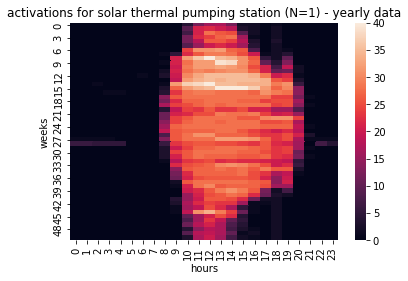
\includegraphics[width=0.9\textwidth]{../Figures/LPS/solar termal pumping station.png}
	\label{fig:solar termal pumping station}
\end{figure}
\begin{figure}[H]
	\centering
	\caption{"Yearly per-appliance light load profile"}
	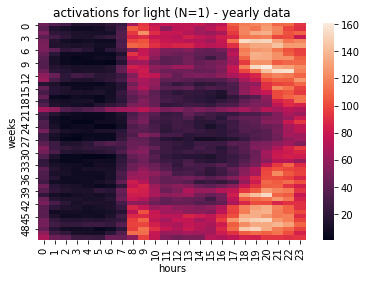
\includegraphics[width=0.9\textwidth]{../Figures/LPS/light.png}
	\label{fig:light}
\end{figure}

Figures \ref{fig:solar termal pumping station} and \ref{fig:light} 
show how weather and season affect the usage pattern of appliances. 

\section{Per-house per-appliance}

The last group of profiles is a combination of per-house and per-appliance load profiles.
Observing the usage pattern of many appliances offers a better look into users usage pattern.
In case of elderly care you would want to observe a group of appliances. Activation of that
group of appliances would yield a contextual event. If stove and kettle are commonly used
together each morning this use could translate to event such as breakfast. 
In order to achieve this one needs to observe all appliances at once such as shown on
figure \ref{fig:PHPA}

\begin{figure}[H]
	\centering
	\caption{"Daily per-appliance per-house building load profile"}
	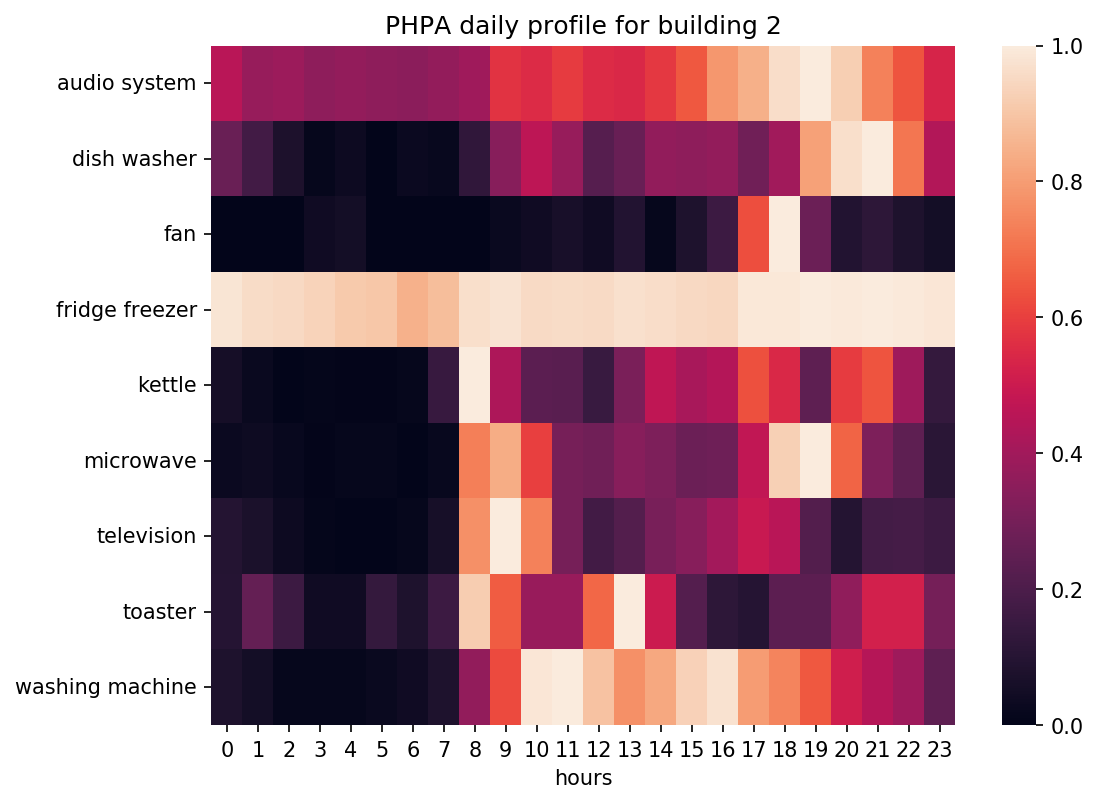
\includegraphics[width=0.9\textwidth]{../Figures/LPS/PHPA.png}
	\label{fig:PHPA}
\end{figure}

The very same data can be presented in alternative way, such as shown on figure \ref{fig:stack}.

\begin{figure}[H]
	\centering
	\caption{"Daily per-appliance per-house building load profile"}
	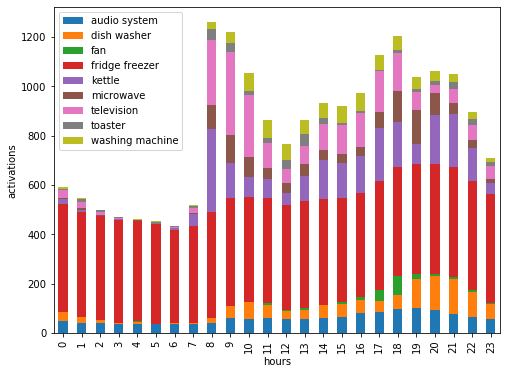
\includegraphics[width=0.9\textwidth]{../Figures/LPS/stack.png}
	\label{fig:stack}
\end{figure}

The usage pattern is the same as on \ref{fig:SLPdaily2}, except that it is possible to see
the contribution of each appliance. 
Altrough these load porfiles are usefull when in comes to analyzeing the usage pattern in one building.
Alternatively it is possible use bag-of-words method from text processing, where a list of most commoly used words is formed,
and then used to process the text. 
Here, It is possibleto use the data from all five datasets and sort the appliances by number of activations.
Only top 30 appliances are seleced. 
Using this list it is possilble to present usage of each building universaly


\begin{figure}[H]
	\centering
	\caption{"Daily per-appliance per-house building load profile"}
	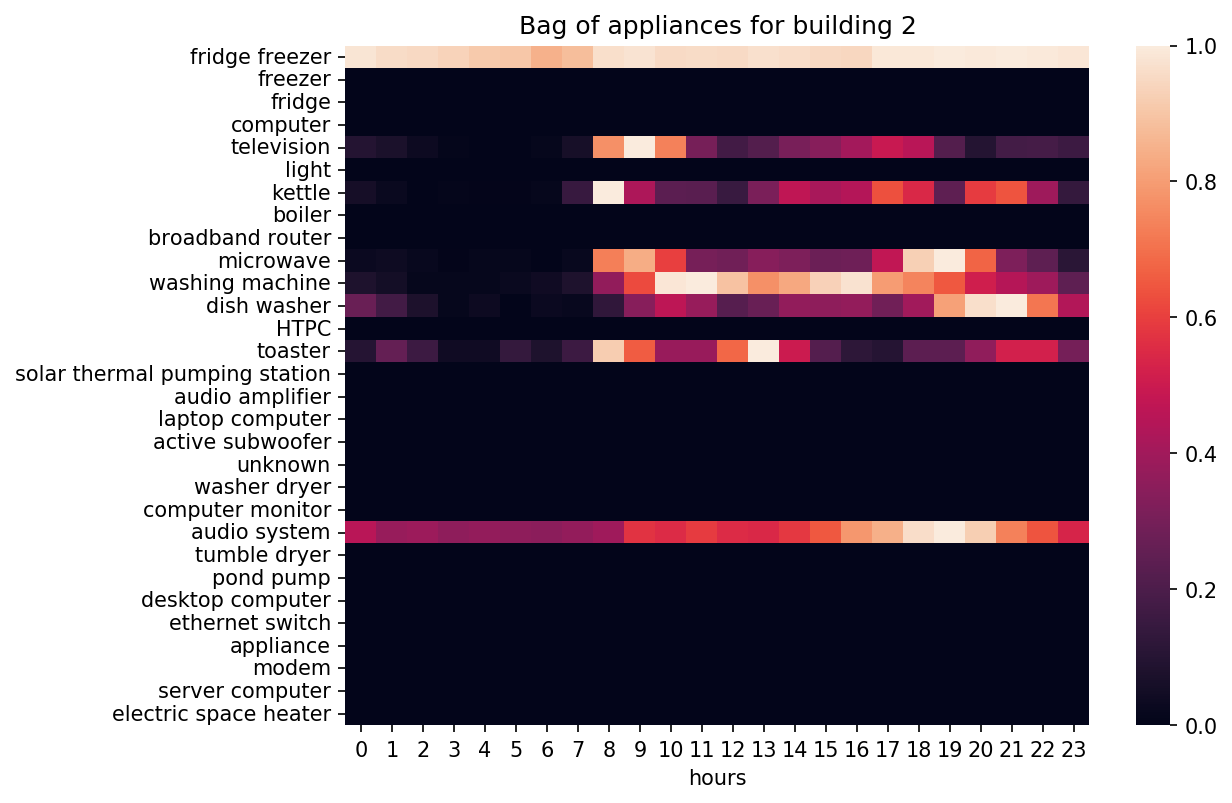
\includegraphics[width=0.9\textwidth]{../Figures/LPS/BOA.png}
	\label{fig:BOA}
\end{figure}


